\documentclass[12pt]{article}
\usepackage{tikz}

\usepackage{graphicx, titling, amsmath, amsthm, amsfonts, amssymb, algorithm, algpseudocode}
\usepackage{tikz}
\usepackage{geometry}
 \geometry{
 a4paper,
 total={170mm,257mm},
 left=20mm,
 top=20mm,
 }
\usepackage{hyperref}

\graphicspath{{./images/}}

% \renewcommand\maketitlehooka{\null\mbox{}\vfill}
% \renewcommand\maketitlehookd{\vfill\null}

\title{DS 221 - Introduction to Scalable Systems: Architectures for AI}
\author{Shankaradithyaa Venkateswaran\\ Sr no: 22190}
\date{\today}

\begin{document}
% \begin{titlepage}
    \maketitle
% \end{titlepage}

\section{Tensor Cores}
\subsection{Introduction}
Tensor cores have emerged as a key component in accelerating artificial intelligence computations, used in deep learning networks. They are specialized hardware units that are designed to perform matrix operations efficiently to speed up AI computations.\\
Tensor cores are found in the NVIDIA architectures where they have become an irreplaceable unit of computation for those architectures. Today I will be taking an indepth look into tensor cores and why they are better than regular GPUs and CPUs for AI computations.

\subsection{What are Tensor Cores?}
Tensor cores are specialized pieces of hardwares found in the NVIDIA Volta, Turing, Ampere, Hopper, and now Blackwell architectures. They are specially designed to perform matrix multiplications efficiently so that they can be used to accelerate deep learning computations.\\
Other companies do not have tensor cores in their GPUs, but they have similar units that perform the same function. For example, AMD has matrix cores in their GPUs that perform the same function as tensor cores. In a later section, I will look into such units in other GPU architectures.\\

\subsection{Features of Tensor Cores}
As I have mentioned above, Tensor cores are designed to perform matrix multiplications efficiently. They are highly specialized compute cores for matrix multiply and accumulate (MMA) math operations. These operations are the core aspect for deep learning computations and HPC.
% \begin{figure}[h]
%     \centering
%     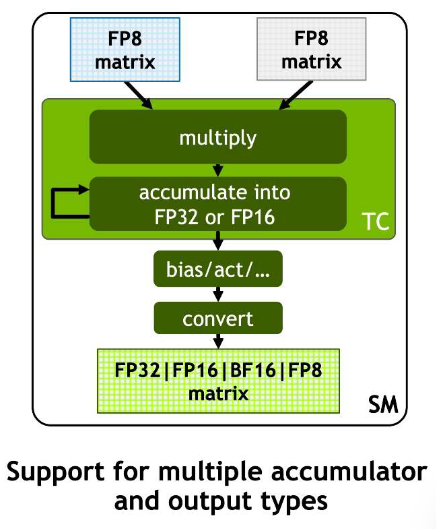
\includegraphics[width=0.5\textwidth]{tensor2.png}
%     \caption{MMA in Tensor Cores; Source: NVIDIA}
% \end{figure}
This operation is to use a lower precision such FP16 (floating point) or INT8 (integer) to perform matrix multiplications and accumulate the results in a higher precision format such as FP32 or FP64. The core multiplies two lower precision matrices and then adds the result to an accumulator matrix which is the same precision or a higher precision. This is then converted to a higher precision format to minimize the loss of precision. This process leads to a preservation of accuracy through the entire process of calculations.
The tensor cores are designed to perform these operations at a very high speed and are capable of performing 64 FMA (fused multiply-add) operations per clock cycle.\\
Tensor cores have a high throughput and low latency, which makes them ideal for AI computations. They are capable of performing 125 teraflops of mixed-precision performance.\\
As we can infer from above, Tensor cores are made to support various datatypes, including FP16, FP32, BF16, INT8, and INT4. This makes them highly versatile and capable of performing a wide range of operations for AI computations.\\
These cores have structured sparsity present in newer architectures such as Ampere and onwards. This means that they can efficiently proccess sparse matrices and ignore the zero values in the matrix. This is a significant improvement over the older architectures where the tensor cores would have to process the zero values as well.\\
Overall, tensor cores are also highly energy efficient to perform matrix calculations on them. They are capable of performing a large number of operations in a short amount of time while consuming less power.

\subsection{Tensor Cores over GPUs and CPUs}
Now the topic comes to why chose tensor cores over GPU and CPU cores. While we can perform AI computations on such cores, it is highly inefficient as CPU and even GPU cores are made with a general purpose use in mind. In the field of a CPU core, it is made to perform a variety of calculations, not just matrix multiplications, hence reducing the efficiency of AI calculations.
Now if we take the example of a GPU core, while it made to perform parallel computations along with matrix operations, it is still not as highly optimized as tensor cores. GPU cores have a variety of other functions as well, rendering pixels, paralle processing, image and video processing, scientific simulations, etc. This means, while they can be used for AI computations, they are not as efficient as tensor cores.\\
Now while CPU and GPU cores can perform matrix multiplications and both of them support MMA in some form or the other, it can safely be said from the statisitcs that tensor cores are much more efficient at performing these operations.
As mentioned above, tensor cores can perform 64 FMA per clock cycle. This is a significant improvement over the regular GPU cores which can perform only 2 FMA operations per clock cycle.\\
Overall, it is just not efficient to run AI or matrix heavy computations on CPU or GPU cores. Tensor cores are highly optimized for these operations and are capable of performing them at a much higher speed and efficiency. Hence it is better to offload such operations to the tensor cores, and clear up space for different operations that are required by the CPU and GPU cores.

% \subsection{DLSS}
% Another example of the efficiency of tensor cores can be seen in the DLSS (Deep Learning Super Sampling) technology by NVIDIA. This is new technology developed by NVIDIA over the past few years, that utilize the full potential of tensor cores. DLSS is used to upscale lower resolution images to a higher resolution using AI.\\
% NVIDIA trains a neural network on a supercomputer to upscale images using AI. This neural network is then used in the tensor cores to upscale the images in real time. This technology is used in games to upscale lower resolution images to a higher resolution in real time.\\
% This could not be possible without the efficiency and speed of tensor cores.

\subsection{Conclusion}
In conclusion, tensor cores are highly efficient and specialized hardware units that are designed to perform matrix multiplications efficiently which directly lead to a collosal speed up in AI computations over the use of regular CPU and GPU cores.

\section{HPC and AI}
Now we will explore the latest state of art HPC architectures tuned for AI. To do this, we will go through three architecture leaders, namely AMD, Intel, and NVIDIA. We will look into their latest architectures and how they are tuned for AI computations.

\subsection{AMD}
AMD has been a leader in the CPU market for a long time now. They have been making strides in the GPU market as well.\\
\textbf{AMD INSTINCT™ MI325X ACCELERATOR}\\
% \begin{figure}[h]
%     \centering
%     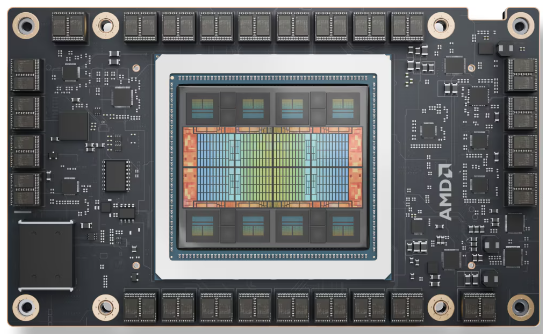
\includegraphics[width=0.5\textwidth]{amd2.png}
%     \caption{ AMD INSTINCT™ MI325X ACCELERATOR; Source: AMD}
% \end{figure}
The figure is a AMD INSTINCT™ MI325X ACCELERATOR designed for increasing demands of AI computations and delievers a amazing HPC performance as well.\\
The discrete AMD Instinct MI325X GPU delievers a superior performance on a broad set of data types needed for AI software, including FP16, BF16, FP8, and INT8. It has an industry leading 256 GB of HBM3E memory and 6 TB/s of memory bandwidth which allows a single acclerator to contain and process a one-trillion parameter model while reducing the cost of ownership for selec LLMs. It has the following performance:\\
\begin{tabular}{c|c|c}
    \hline
    AI Peak Performance & without sparsity & with sparsity\\
    \hline
    TF32 (TFLOPs) & 653.7 & 1307.4\\
    FP16 (TFLOPs) & 1307.4 & 2614.9\\
    BFLOAT16 (TFLOPs) & 1307.4 & 2614.9\\
    INT8 (TOPs) & 2614.9 & 5229.8\\
    FP8 (TFLOPS) & 2614.9 & 5229.8\\
    \hline
    HPC Peak Performance & & \\
    \hline
    FP64 vector (TFLOPs) & 81.7 & NA\\
    FP32 vector (TFLOPs) & 163.4 & NA \\
    FP64 matrix (TFLOPs) & 163.4 & NA \\
    FP32 matrix (TFLOPs) & 163.4 & NA\\
\end{tabular}\\
% \begin{itemize}
%     \item AI Peak performance
%     \begin{itemize}
%         \item TF32 (TFLOPs) 653.7 and 1307.4 with sparsity.
%         \item FP16 (TFLOPs) 1307.4 and 2614.9 with sparsity.
%         \item  BFLOAT16 (TFLOPs) 1307.4 and 2614.9 with sparsity.
%         \item INT8 (TOPs) 2614.9 and 5229.8 with sparsity.
%         \item  FP8 (TFLOPS) 2614.9 and 5229.8 with sparsity.
%     \end{itemize}
%     \item HPC Peak performance
%     \begin{itemize}
%         \item FP64 vector (TFLOPs) 81.7
%         \item FP32 vector (TFLOPs) 163.4
%         \item FP64 matrix (TFLOPs) 163.4
%         \item FP32 matrix (TFLOPs) 163.4
%     \end{itemize}
% \end{itemize}
The AMD Instinct MI325X accelerator is an AMD CDNA 3 architcture-based accelerator with high throughput based on improved AMD Matrix cores. Matrix cores are the equivalent of tensor cores in NVIDIA GPUs. They are designed to perform matrix multiplications efficiently.\\
Each discrete MI325X GPU offers a 16-lane host interface with PCIe Gen 5 support, enabling high-speed data transfer between the host and the accelerator.\\
The features of the MI325X accelerator which accelerate AI computations can be broadly described as the increased memory bandwidth and the memory capacity of the accelerator. The architecture itself is purpose built to drive the most demanding AI computations. The specifications include:\\
\begin{tabular}{c|c}
    \hline
    Feature & Capacity\\
    \hline
    Form factor & OAM (Open Accelerator Module)\\
    GPU compute units & 304\\
    Matrix cores & 1216\\
    Stream processors & 19,456\\
    Peak Engine Clock & 2100 MHz\\
    Memory Capacity & Up to 356 GB\\
    Memory Bandwidth & 6 TB/s (peak theoretical)\\
    Memory Interface & 8192-bit HBM3E\\
    PCIe Gen 5 x16 & 128 GB/s\\
    Infinity Fabric Link & 7x 128 GB/s\\
    \hline
\end{tabular}\\
% \begin{itemize}
%     \item Form factor: OAM (Open Accelerator Module)
%     \item GPU compute units: 304
%     \item Matrix cores: 1216
%     \item Stream processors: 19,456
%     \item Peak Engine Clock: 2100 MHz
%     \item Memory Capacity: Up to 356 GB
%     \item Memory Bandwidth: 6 TB/s (peak theoretical)
%     \item Memory Interface: 8192-bit HBM3E
%     \item PCIe Gen 5 x16 (128 GB/s)
%     \item Infinity Fabric Link: 7x 128 GB/s
% \end{itemize}
the infinity fabric link is a high-speed interconnect that allows for high-speed data transfer between the GPUs. Each OAM module includes: Eight accelerated compute dies (XCDs) with 38 compute units (CUs), 32 KB of L1 cache per CU, 4 MB shared L2 cache shared across CUs, and 256 MB of AMD Infinity Cache™ shared across 8 XCDs.\\
% \begin{itemize}
%     \item 
%     \item 
%     \item 
%     \item  
% \end{itemize}
These compute units support a broad range of precisions for both AI/ML and HPC acceleration, native hardware support for sparsity, and enhanced computations throughput. The OAM also includes: Four supported decoders for HEVC/H.265, AVC/H.264, VP9, or AV1, each with an additional 8-core JPEG/MPEG CODEC, 256 GB of HBM3E memory with 6 TB/s on-package peak throughput, and SR-IOV for up to 8 partitions.\\
% \begin{itemize}
%     \item 
%     \item 
%     \item 
% \end{itemize}
(Note: I did not go too indepth into the above terms)\\
AMD has also introduced the ROCm (Radeon Open Compute) platform which is an open-source software platform that allows for the development of high-performance computing and AI applications. It is designed to work with AMD GPUs and accelerators. All these combine to form an architecture that is highly optimized for AI computations and HPC. Now these AMD MI325X accelerators can be stacked on each other on a AMD Universal Base Board (UBB 2.0) with HGX host connecters to form the AMD Instinct MI300X MI325X Platform.

% \subsubsection{AMD INSTINCT™ MI325X PLATFORM}
% This is a 8 GPU platform that is designed to deliver the highest performance for AI and HPC workloads.\\
% \begin{figure}[h]
%     \centering
%     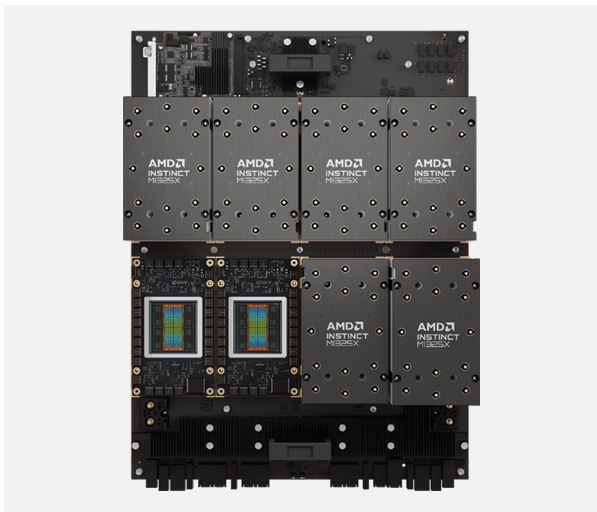
\includegraphics[width=0.5\textwidth]{amd3.png}
%     \caption{ AMD INSTINCT™ MI325X PLATFORM; Source: AMD}
% \end{figure}
% With this architecture we get the following performance:
% \begin{itemize}
%     \item AI Peak performance
%     \begin{itemize}
%         \item TF32 (PFLOPs) 5.2 and 10.5 with sparsity.
%         \item FP16 (PFLOPs) 10.5 and 20.9 with sparsity.
%         \item  BFLOAT16 (PFLOPs) 10.5 and 20.9 with sparsity.
%         \item INT8 (POPs) 20.9 and 41.8 with sparsity.
%         \item  FP8 (PFLOPS) 20.9 and 41.8 with sparsity.
%     \end{itemize}
%     \item HPC Peak performance
%     \begin{itemize}
%         \item FP64 vector (TFLOPs) 653.6
%         \item FP32 vector (PFLOPs) 1.3
%         \item FP64 matrix (PFLOPs) 1.3
%         \item FP32 matrix (PFLOPs) 1.3
%     \end{itemize}
% \end{itemize}
% As we can see, combining 8 MI325X accelerators on a single platform gives a significant boost in performance. This entire platform is connected by the AMD Infinity Fabric Link which allows for high-speed data transfer between the GPUs. The fully meshed 128 GB/s bidirectional links between the MI325X GPUs along with PCLe Gen 5 x16 I/O conectivity allows for high-speed data transfer between the GPUs and GPUs and GPUs and the host.
% \begin{figure}[h]
%     \centering
%     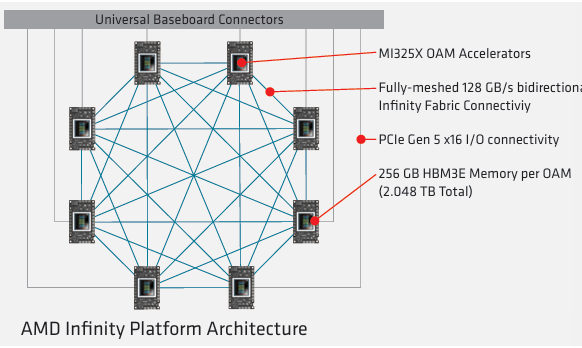
\includegraphics[width=0.5\textwidth]{amd4.png}
%     \caption{ AMD Infinity Platform Architecture: AMD}
% \end{figure}
% Compiling 8 MI325X accelerators on a single platform makes the specifications such as GPU compute units, matrix cores, stream processors, and memory capacity octuple in size.\\
% All these specifications with high speed interconnectivity between the MI325X accelarators make this platform a beast of a processor for HPC tuned for Ai computations.

\subsection{Intel}
Moving on let us now talk about Intel and their latest architecture for HPC which are tuned for AI computations. Intel, just like AMD has made its own language to support HPC which is called the oneAPI. This supports HPC standards including C/C++, Fortran, Python, OpenNP, and MPI for integration.

% \subsubsection{Intel® Xeon® CPU Max Series}
% Lets start out by talking about the Intel Xeon CPU Max Series. This is a series of CPUs that are designed to deliver the highest performance for AI and HPC workloads from Intel.\\
% This is the only x86-based processor with high bandwidth memory from Intel to deliever the best HPC and AI performance.\\
% The Intel Max series CPUs feature:
% \begin{itemize}
%     \item 56 performance cores
%     \item  64 GB of high bandwidth in-package memory
%     \item PCI Express 5.0 bandwidth
%     \item Peak HBM transfer rate:  3200 MT/s
%     \item Accelerators: AMX, 4 DSA Devices
%     \item AI/ML Instructions: BF16 and INT8
% \end{itemize}
% These ccores will provide memory (HBM) capcity per core, enough to fit most HPC workloads.
% While these are CPUs, they are designed to provide the flexibility to run a wide range of workloads, including AI and HPC.\\
% \begin{itemize}
%     \item HBM-Only MOde: This mode used all 64 GB of capacity and ability to scale at 1-2 GB memory per core.
%     \item HBM Flat Mode: this provides the flexibility for applications that require large memory capacity. It provides a flat memory region with HBM and DRAM and works with workloads requiring larger than 2 GB per core.
%     \item HBM Cache Mode: This mode is designed for applications that require a large cache. It works for workloads with greater than 64 GB capacity and/or requiring greater than 2 GB per core.
% \end{itemize}
% Another noteworthy advancement for the Intel Xeon CPU Max Series is the AMX (Advanced Matrix Extensions) which is a new set of instructions that are designed to accelerate matrix operations. This is similar to the tensor cores in NVIDIA GPUs and matrix cores in AMD GPUs.

\textbf{Intel® Data Center GPU Max Series}\\
Like the Intel® Xeon® CPU Max Series we have the Intel® Data Center GPU Max Series. The previous code name of this series was the Ponte Vecchio.\\
This GPU product is based on the Intel $X^{e}$ HPC micro-architecture. The GPu takes advantage of highly parallelized computing models associated with AI and HPC. Just like the CPU max series, the GPU max series is supported by the oneAPI open exosystem with the flexibility of Single Instruction Multiple Data (SIMD) and Single Instruction Multiple Thread (SIMT) programming models.\\
% \begin{figure}[h]
%     \centering
%     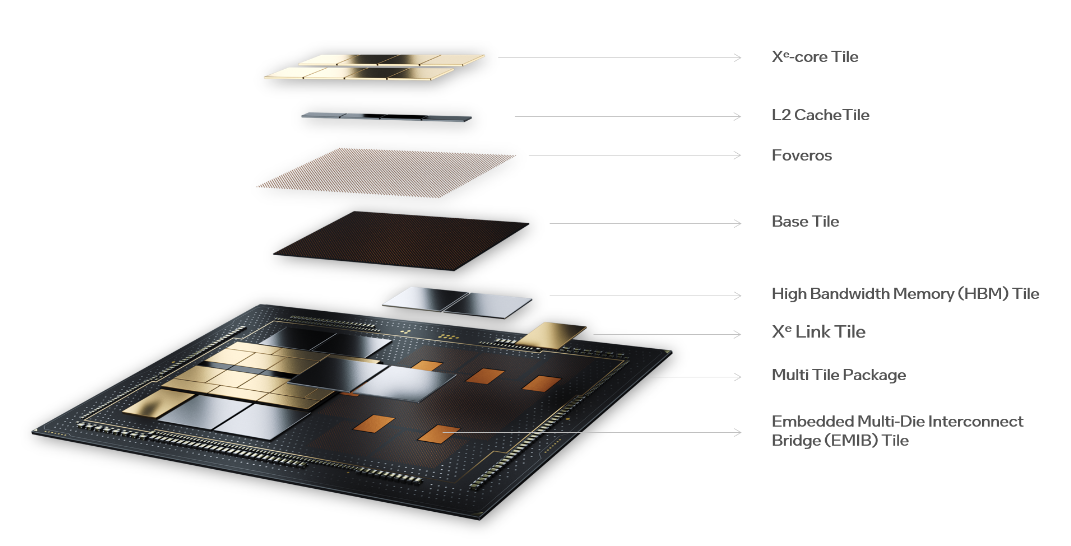
\includegraphics[width=0.5\textwidth]{intel1.png}
%     \caption{ $X^{e}$ HPC Stack; Source: Intel}
% \end{figure}
The heart of the product is the Intel $X^{e}$ HPC stack. The components of the stack are as shown in the above figure. All these components reside within a Multi Tile Package.\\
This GPU will have OAM modules, just like the AMD MI325X accelerators. The Max Series 1350 GPU has a 450W TDP and 96GB of HBM2e memory. It will have 112 $X^{e}$ cores.\\
The larger OAM module will have full 600 W 128 GB HBM2e memory and a full 128 $X^{e}$ cores. All this will be called the Max Series 1550 GPU.\\
To link these OAM modules, Intel has its own connection system called the Intel $X^{e}$ Link. 
These links will provide high speed interconnects between the OAMs to provide high performance for AI and HPC workloads.\\
Both tehe Max Series 1350 and 1550 GPUs are connected with the PCI express 5.0 interface and with both of them having up to 4x HBM2e 3.2GT/s\\
The performances of each are as follows:\\
\begin{tabular}{c|c|c}
    \hline
    & Max Series 1350 & Max Series 1550\\
    \hline
    FP64 PEAK FLOPS & 44 TFLOPS & 52 TFLOPS\\
    FP32 PEAK FLOPS & 44 TFLOPS & 52 TFLOPS\\
    BF16 PEAK FLOPS & 832 FLOPS & 704 TFLOPS\\
    INT8 PEAK FLOPS & 1664 TFLOPS & 1408 TFLOPS\\
    \hline
\end{tabular}\\
Overall the performance of the Intel Data Center GPU Max Series is comparable to other GPUs in the market.

\subsection{NVIDIA}
Finally, we come to NVIDIA. NVIDIA has been a leader in the GPU market for a long time now. We will dive into their latest architectures and see what makes them the leaders of the AI and HPC market.

\textbf{NVIDIA Hopper Architecture}\\
NVIDIA's Hopper architecture is the latest architecture from NVIDIA on the market. It is stated to securely deliver the highesh performance computing with lowe latency.\\
% \begin{figure}[h]
%     \centering
%     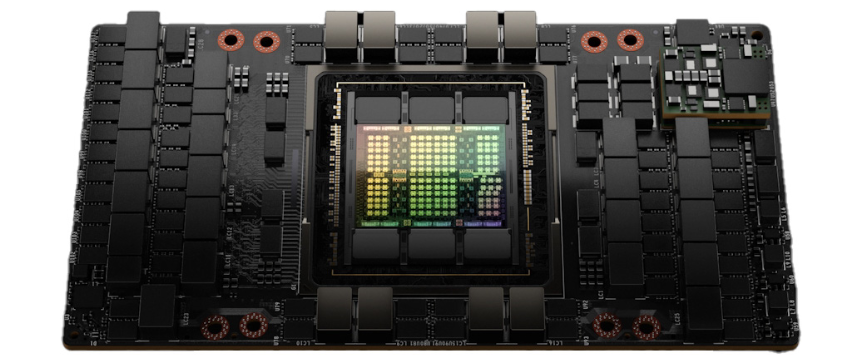
\includegraphics[width=0.5\textwidth]{nvidia1.png}
%     \caption{NVIDIA Hopper Architecture; Source: NVIDIA}
% \end{figure}
The H100 is NVIDIA's 9th generation data center GPU designed for AI and HPC. It is magnitudes faster thatn the prior generation NVIDIA A100. The H100 carries over the major design focus of A100 and improved the strong scaling for AI and HPC workloads. The following are the results of benchmarking the H100 against the A100.
% \begin{figure}[h]
%     \centering
%     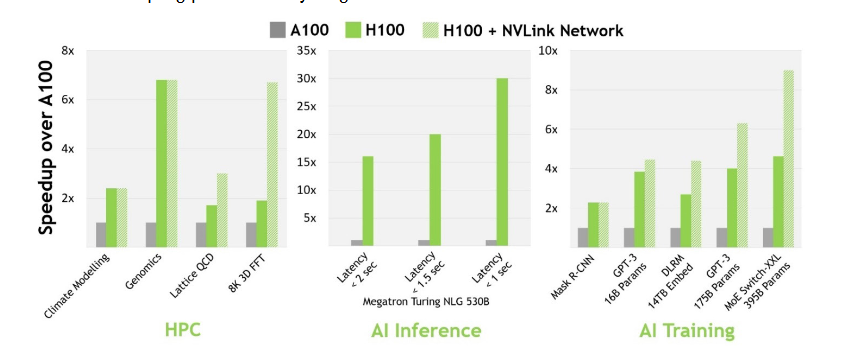
\includegraphics[width=\textwidth]{nvidia2.png}
%     \caption{NVIDIA H100 vs A100; Source: NVIDIA}
% \end{figure}
The H100 has multiple new features and improvements over the A100.
% here I will only go over the key features which boost the HPC performance and AI computations. 
These features are:
\begin{itemize}
    \item New Streaming Multiprocessor:
    \begin{itemize}
        \item New fourth generation Tensor Cores which are upt o 6x faster chip to chip compared to A100, including per SM speedup, additional SM count, adn higher clocks of H100. Overall, this a giant upgrade to the A100 as we have seen that tensor cores are vital for AI computations, and the H100 is just better at it than the A100. 
        %There are multiple other improvements such as better MMA computations rates per SM, and an implemented sparsity feature to exploit fine grained structeures sparsity in deep neural networks.
        \item 3x faster IEEE FP64 and FP32 processing raters chip to chip compared to A100.
        \item New thread block cluster feature which allows programmiatically control of a localily at a granularity larger than a single Thread block on a single SM. 
        %This directly feeds into the efficacy of CUDA programming giving more freedom and adding another level of the programming hierarchy.
        \item A new Asynchronous Execution to enable a new Tensor Memory Accelerator (TMA) to transfer larger blocks of data efficiently between global memory and shared memeory. I need not say how important this is for offloading large datasets for AI computations.
    \end{itemize}
    \item New Transformer Engine:\\
    The H100 has a new transformer engine which is a combination of software and custom Hopper Tensor COre technology which directly accelerates Transformer model training and inferences. 
    %It does this by intelligently managing and dynamically choosing between FP8 and 16 calculations to maximize performance at each layer. 
    This lets it deliver up to 9x faster AI training and up to 30x faster AI inference speedups on LLMs compared to A100.
    \item HBM3 Memory:\\
    The H100 provides a 2x bandwidth increase compared to A100. As stated by NVIDIA, teh H100 SXM5 GPU is the world's first GPU with HBM3 memory delivering a class-leading 3 TB/sec of memory bandwidth. 
    %This is obviously a feature required both in HPC and AI computations.
    \item The H100 has a 50MB L2 cache which caches large portions of models and datasets for repeated access.
\end{itemize}
% The H100 has many other improvements over connections becoming faster compared to the A100 causing the connections between the GPU cores to become more streamlined and the connection between the GPU and the base to get stronger and faster as well. But if I keep listing them, it will take even more time than necessary. For now, I have listed the important features which promote HPC tuned for AI. 
The performances of the H100 are given below:\\
\begin{center}
\begin{tabular}{c|c|c}
    \hline
    & H100 SXM5 & H100 SXM5 Sparse\\
    \hline
    FP8 tensor core & 1978.9 TFLOPS & 3957.8 TFLOPS\\
    FP16 & 133.8 TFLOPS & NA\\
    FP16 tensor core & 989.4 TFLOPS & 1978.9 TFLOPS\\
    BF16 tensor core & 989.4 TFLOPS & 1978.9 TFLOPS\\
    FP32 & 66.9 TFLOPS & NA\\
    TF32 tensor core & 494.7 TFLOPS & 989.4 TFLOPS\\
    FP64 & 33.5 TFLOPS & NA\\
    FP64 tensor core & 66.9 TFLOPS & NA\\
    INT8 tensor core & 1978.9 TFLOPS & 3957.8 TFLOPS\\
\end{tabular}\\
\end{center}
From this table we can clearly see that tensor cores accelerate the computations, which makes this architecture perfect for both HPC And AI.\\
The H100 is an engineering marvel which promote HPC and AI, but to truly boost our HPC and dig deep for AI we need to go even further beyond.

\textbf{NVIDIA DGX}\\
This is NVIDIA's foundational building block for Data centers for AI. The DGX system uses chips such as the A100 to build a foundational block that can handle large scale computations and, well, HPC. With each generation the DGX can get upgraded with a new chip. Here I will talk about the NVIDIA DGX H100. This is the version of NVIDIA's DGX system with the H100 chip.\\
The NVIDIA DGX H100 has the following specifications to boost HPC for AI specific tasks:\\
\begin{tabular}{c|c}
    \hline
    Feature & Capacity\\
    \hline
    GPU & 8x H100 Tensor Core GPUs\\
    Tensor Cores & 4th gen Tensor Cores with sparsity handling\\
    NVLink & 4th gen NVLink (connections inside the chips)\\
    NVSwitch & 4x - 3rd gen NVSwitch\\
    ConnectX & 8x ConnectX - 7 (400 GB/s InfiniBand / Ethernet)\\
    DPU & 2x Bluefield 3- DPUs\\
    PCIe & PLCe Gen5\\
    \hline
\end{tabular}\\
% \begin{itemize}
%     \item 8x H100 Tensor Core GPUs
%     \item 4th gen Tensor Cores with sparsity handling
%     \item 4th gen NVLink (connections inside the chips)
%     \item 4x - 3rd gen NVSwitch
%     \item 8x ConnectX - 7 (400 GB/s InfiniBand / Ethernet)
%     \item 2x Bluefield 3- DPUs
%     \item PLCe Gen5
% \end{itemize}
This type of architecture allows for insane data center scalability which is why it is one of the top options in the market today.
% Now that we have talked about NVIDIA's data center chips, lets talk about another architecture, namely the ARM Architecture.

% \subsubsection{Grace Chips}
% The Grace chip is NVIDIA's first datacenter CPU. It comprises of system-on-chip(SoC) that has 72 high-performance ARM v9 cores and feature the Scalable Coherency Fabric (as stated by NVIDIA). As it is using the ARM architecture, Grace provides a high performance compute foundation in a low power system-on-chip.\\
% Grace is, by no means, lagging behind other CPU chips. It is build on standarsd such as Arm SystemReady and is compatible with a wide variety of Arm-compatible operating systems, PCIe, and USB peripherals, drivers, and application softwares.\\
% Now this may all seem impressive for a cpu chip, but how is it relevant for HPC or even AI?\\
% Well the answer or the magic comes in the next section, which is where we combine the two powerhouses to create something extraordinary.

% \subsubsection{Grace-Hopper Superchip}
% NVIDIA has combined two of the most powerful and efficient CPU and GPU chips into one unit to create the Grace-Hoopper Superchip. This is called the NVIDIA GH200, it brings together the performances of both the G100 and the H100 chips to create something magical.\\
% \begin{figure}[h]
%     \centering
%     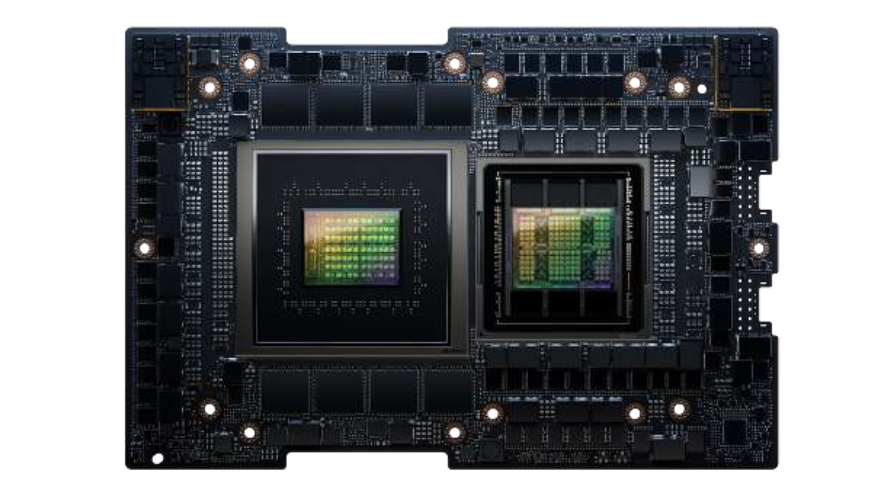
\includegraphics[width=0.5\textwidth]{nvidia3.png}
%     \caption{NVIDIA Grace-Hopper Architecture; Source: NVIDIA}
% \end{figure}
% It is interconnected by the NVIDIA NVline-C2C which is NVIDIA's memory coherent, high-bandwidth, and low latency interconnect for superchips. As stated by NVIDIA, it is the heart of the GH200 and delivers up to 900 GB/s total bandwidth. This is 7x higher bandwidth tahn x16 PCIe Gen5 lanes.\\
% The point of this new interconnect is to increase the performance of the GH200 by keeping all the threads and cores busy whenever possible. It allows the chip to intelligently and effiectively delegate tasks to sperate parts and combine the information outputted at a moments notice.\\
% The GH200 uses 96GB of HBM3 memory, delivering 4TB/s of memory bandwidth. The GH200 has some other specifications as well that improve performance over just using a G100 or a H100 chip, but I will not go over these.\\
% Overall the GH200 takes the goodness of both the G100 and the H100 and utilizes both of them to the max with the necessary high speed interconnects to achieve a different level of HPC tuned for AI.

% \subsubsection{Blackwell}
% Recently, this year, NVIDIA announced the Blackwell architecture, which takes all the specifications of the Hopper architecture and amp it up to a new realm.\\
% The Blackwell architecture uses 208 billion transistors, more than 2.5x the transistors of the Hopper architecture, and thats not all. It has the second generation Transformer engine which allows it to supercharge the inference of large MoE models, add new precisions, and introduce a dynamic range of algorithms to chose between to get the best scaling and accuracy from the computations possible.\\
% The 2nd generation transformer engine also works with the Nemo Frameword and the Megatron-Core innovations to experly parallelize operations to further acclerate AI computations for training and inferences.\\
% The Blackwell architcture also has the fifth generation NVline and NVLink Switch. These new links greatly decrease the communication times between every GPu within a server cluster.\\
% The fifth generation of NVLink can scale up to 576 GPUs to accelerate performance for trillion- and multi-trillion-parameter AI models thanks to the NVLink Switch ASIC and switches built with it.\\
% Blackwell GPUs include 18 fifth generation NVlinks to provide 1.8 TB/sec total bandwidth, 900 GB/sec in each direction. This is an insane number which is nearly 7 petabytes of data transfer in an hour for 1 gpu, or more data than 18 years of streaming 4k movies, or the entire internet bandwidth processed by just \textbf{11} Blackwell GPUs.\\
% The Blackwell GPUs also have a new and improved Decompression system which helps in processing database queries quickly and effectively. It is 6x faster than the H100 chips for query benchmarks.\\
% \begin{figure}[h]
%     \centering
%     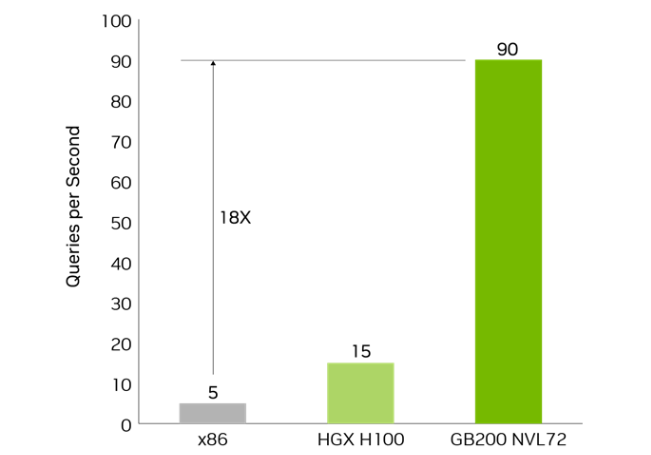
\includegraphics[width=0.5\textwidth]{nvidia4.png}
%     \caption{Blackwell vs hopper; Source: NVIDIA}
% \end{figure}
% Finally to top it all off, the Blackwell architecture has a RAS Engine which adds intelligent resiliency. This allows the chip to identify potential faults that may occus early on to minimize downtime. This is an AI-powered predictive management that continuously montiors thousands of datapoints across hardware and software to predict and intercept sources of downtime and inefficiency. This directly helps in HPC and AI which is what the Blackwell chip is made for.\\
% Now that I have laid out the broad details of the Blackwell architcture and why it is much better than the Hopper architcture, we can now build on top of these with the following.\\
% The DGX architecture can also take the B100 chips and have the same performance increases relative to just one B100 just as I discussed previously.\\
% \begin{figure}[h]
%     \centering
%     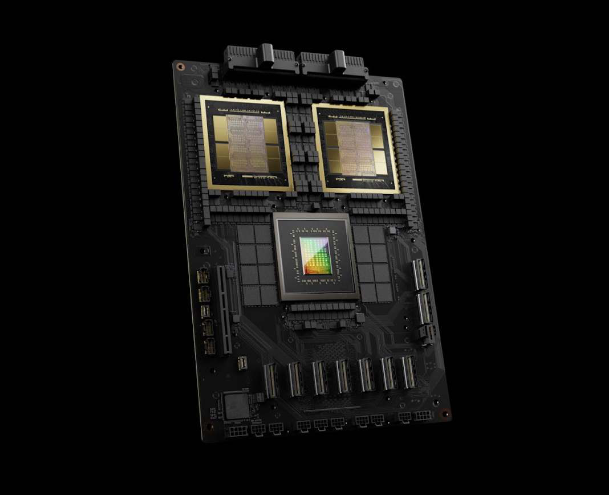
\includegraphics[width=0.5\textwidth]{nvidia5.png}
%     \caption{NVIDIA GB200; Source: NVIDIA}
% \end{figure}
% Moving on, we can also configure the Grace-Blackwell Superchip. This chip uses 1 Grace CPU and 2 Blackwell GPUs to give a terrifying performance unlike anything I've ever seen.\\
% This can be further upgraded to the NVIDIA GB200 NVL 72, which connects 36 GB200 superchips in a rack-scale design. This cluster has to be liquid cooled and acts as a massive GPU to deliever 30x faster real0time trillion parameter LLM inference than the prior generation.\\
% \begin{figure}[h]
%     \centering
%     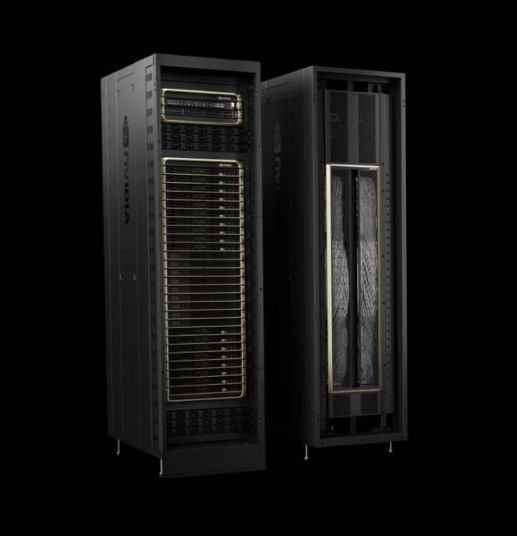
\includegraphics[width=0.5\textwidth]{nvidia6.png}
%     \caption{NVIDIA GB200 NVL 72; Source: NVIDIA}
% \end{figure}
% It is projected to deliever 30 times more output tokens per second per GPU than the HGX H100.\\
% As the performances and specifications are still subject to change, I will not be including these in this report. 

\textbf{Conclusion}\\
This is the end of my report on Tensors cores and why they are helpful for AI and the different architecture leaders and their leading architecutres for HPC tuned for AI.

\section{References}
\href{https://developer.nvidia.com/blog/structured-sparsity-in-the-nvidia-ampere-architecture-and-applications-in-search-engines/#:~:text=NVIDIA%20Ampere%20and%20NVIDIA%20Hopper%20architecture%20GPUs%20add,Tensor%20Cores%2C%20which%20require%20a%202%3A4%20sparsity%20pattern}{Sparsity Docs from NVIDIA}\\
\href{https://medium.com/@rowanbrooks.cloudies/cuda-cores-vs-tensor-cores-which-one-is-right-706275ffc1aa}{Medium Article on Tensor Cores}\\
\href{https://developer.download.nvidia.com/video/gputechconf/gtc/2020/presentations/s21929-tensor-core-performance-on-nvidia-gpus-the-ultimate-guide.pdf}{Tensor Core Slides by NVIDIA}\\
\href{https://www.trustedreviews.com/explainer/what-are-tensor-cores-4422136}{Tensor Cores Article}\\
\href{https://www.nvidia.com/en-us/data-center/tensor-cores/}{Tensor Core docs from NVIDIA}\\
\href{https://resources.nvidia.com/en-us-tensor-core}{Hopper Whitepaper}\\
\href{https://www.nvidia.com/content/dam/en-zz/Solutions/Data-Center/nvidia-dgx-a100-datasheet.pdf}{DGX A100 Datasheet from NVIDIA}\\
\href{https://docs.nvidia.com/dgx-systems/index.html}{DGX Docs from NVIDIA}\\
\href{https://www.amd.com/content/dam/amd/en/documents/instinct-tech-docs/product-briefs/instinct-mi325x-datasheet.pdf}{AMD Instinct MI325X Datasheet}\\
\href{https://www.servethehome.com/new-intel-data-center-gpu-max-at-sc22-including-pcie-and-oam/}{Article on Intel Data Center GPU Max Series}\\
\href{https://www.intel.com/content/www/us/en/products/sku/232876/intel-data-center-gpu-max-1100/specifications.html}{Intel Data Center GPU Max Series Docs from Intel}\\
\href{https://www.intel.com/content/www/us/en/developer/articles/technical/intel-data-center-gpu-max-series-overview.html}{Intel Data Center GPU Max Series Overview from Intel}\\
\href{https://www.storagereview.com/news/intel-xeon-cpu-max-series-and-intel-data-center-gpu-max-series-introduced}{Article Introducing Intel Xeon CPU Max Series and Intel Data Center GPU Max Series}\\
\href{https://www.intel.com/content/www/us/en/developer/topic-technology/high-performance-computing/overview.html}{HPC docs from Intel}
% \begin{itemize}
%     \item \href{https://developer.nvidia.com/blog/structured-sparsity-in-the-nvidia-ampere-architecture-and-applications-in-search-engines/#:~:text=NVIDIA%20Ampere%20and%20NVIDIA%20Hopper%20architecture%20GPUs%20add,Tensor%20Cores%2C%20which%20require%20a%202%3A4%20sparsity%20pattern}{Sparsity Docs from NVIDIA}
%     \item \href{https://medium.com/@rowanbrooks.cloudies/cuda-cores-vs-tensor-cores-which-one-is-right-706275ffc1aa}{Medium Article on Tensor Cores}
%     \item \href{https://developer.download.nvidia.com/video/gputechconf/gtc/2020/presentations/s21929-tensor-core-performance-on-nvidia-gpus-the-ultimate-guide.pdf}{Tensor Core Slides by NVIDIA}
%     \item \href{https://www.trustedreviews.com/explainer/what-are-tensor-cores-4422136}{Tensor Cores Article}
%     \item \href{https://www.nvidia.com/en-us/data-center/tensor-cores/}{Tensor Core docs from NVIDIA}
%     \item \href{https://resources.nvidia.com/en-us-tensor-core}{Hopper Whitepaper}
%     \item \href{https://www.nvidia.com/en-us/data-center/grace-cpu/}{Grace CPU Page from NVIDIA}
%     \item \href{https://docs.nvidia.com/grace/index.html}{Grace Docs from NVIDIA}
%     \item \href{https://resources.nvidia.com/en-us-grace-cpu/nvidia-grace-hopper?ncid=no-ncid}{Grace Hopper Whitepaper}
%     \item \href{https://www.nvidia.com/en-us/data-center/gb200-nvl2/?ncid=no-ncid}{Grace Blackwell Docs from NVIDIA}
%     \item \href{https://resources.nvidia.com/en-us-blackwell-architecture?ncid=no-ncid}{Blackwell Whitepaper}
%     \item \href{https://www.nvidia.com/en-us/data-center/gb200-nvl72/?ncid=no-ncid}{GB200 NVL 72 Docs from NVIDIA}
%     \item \href{https://www.nvidia.com/content/dam/en-zz/Solutions/Data-Center/nvidia-dgx-a100-datasheet.pdf}{DGX A100 Datasheet from NVIDIA}
%     \item \href{https://docs.nvidia.com/dgx-systems/index.html}{DGX Docs from NVIDIA}
%     \item \href{https://www.amd.com/en/products/accelerators/instinct/mi300/mi325x/platform.html}{AMD Instinct MI325X Platform docs from AMD}
%     \item \href{https://www.amd.com/content/dam/amd/en/documents/instinct-tech-docs/product-briefs/instinct-mi325x-platform-datasheet.pdf}{AMD Instinct MI325X Platform Datasheet}
%     \item \href{https://www.amd.com/content/dam/amd/en/documents/instinct-tech-docs/product-briefs/instinct-mi325x-datasheet.pdf}{AMD Instinct MI325X Datasheet}
%     \item \href{https://www.servethehome.com/new-intel-data-center-gpu-max-at-sc22-including-pcie-and-oam/}{Article on Intel Data Center GPU Max Series}
%     \item \href{https://www.intel.com/content/www/us/en/products/sku/232876/intel-data-center-gpu-max-1100/specifications.html}{Intel Data Center GPU Max Series Docs from Intel}
%     \item \href{https://www.intel.com/content/dam/www/central-libraries/us/en/documents/2023-01/xeon-cpu-max-series-product-brief.pdf}{Intel Xeon CPU Max Series product brief from Intel}
%     \item \href{https://www.intel.com/content/www/us/en/developer/articles/technical/intel-data-center-gpu-max-series-overview.html}{Intel Data Center GPU Max Series Overview from Intel}
%     \item \href{https://www.storagereview.com/news/intel-xeon-cpu-max-series-and-intel-data-center-gpu-max-series-introduced}{Article Introducing Intel Xeon CPU Max Series and Intel Data Center GPU Max Series}
%     \item \href{https://www.intel.com/content/www/us/en/developer/topic-technology/high-performance-computing/overview.html}{HPC docs from Intel}
% \end{itemize}

\textbf{Disclaimer:}\\
While completing this report, the teams message requiring the document to be at max 6 pages was sent. I have had to cut out a tremendous portion of whatever I wanted to report in response to make the document fit the requirements. Thank you for understanding.
\end{document}
